\section{Infinite Series}
\subsection{Geometric Series}
In the first chapter, consideration of $\frac{1}{3}=0.333\cdots$ led us to the sequence
\[
a_n  = \frac{3}{10} + \frac{3}{100} + \cdots + \frac{3}{10^{n-1}} + \frac{3}{10^n}
\]
i.e. defining $a_n$ as the sum of the first $n$ terms of another sequence, here $b_k=\frac{3}{10^k}$.  We now fulfill our promise that we would see other sequences defined in this way.
So we introduce some notation for sequences defined by ever-longer sums.
\begin{defn}\label{def:infSer}
Given any sequence $b_n$ we define the \emph{infinite series}
\[
\sum_{k=0}^{\infty} b_k
\]
to mean
\[
\lim_{n \to \infty} b_0+b_1+b_2+ \cdots + b_n
\]
if the limit exists (in which case we say the series is convergent). Sums of the form $\sum_{k=0}^{n} b_k = b_0+b_1+b_2+ \cdots + b_n$ are called \emph{partial sums} of the infinite series.
\end{defn}

The most fundamental example of a convergent series is known as the \emph{geometric series}: 
\begin{thm}\label{thm:geometricSeries}
For any $-1<x<1$,
\[
\sum_{k=0}^{\infty} x^k = 1 + x + x^2 + \cdots = \frac{1}{1-x}
\]
\end{thm}
\begin{proof}
Before proving the theorem, note that with $x=\frac{1}{10}$ it becomes
\[1.1111\cdots = \frac{10}{9}\]
which is just a mild tweaking of the classic $0.333\cdots = \frac{1}{3}$.

We both demonstrate that the series converges and determine its value by finding an explicit expression for the $k^{\mbox{th}}$ partial sum
\[
a_k(x) = 1 + x + x^2 + \cdots + x^k
\]
The trick is to note how nicely this expression can be manipulated into variations of itself. In particular, multiplying by $x$ only changes the first and last terms: $xa_k(x) = a_k(x) - 1 + x^{k+1}$, thus
\[
a_k(x) = \frac{1-x^{k+1}}{1-x}
\]
and the result follows from theorem \ref{thm:geometricLim}, which tells us that $\lim x^k = 0$.
\end{proof}

It is sometimes convenient to drop the $k=0$ term (which is not very interesting since it is always 1 regardless of $x$) and write
\[
\sum_{k=1}^{\infty} x^k = x + x^2 + x^3 +\cdots = \frac{1}{1-x} - 1 = \frac{x}{1-x}
\]
A noteworthy  special case is $x=1/2$, i.e.
\begin{equation}\label{eq:Zeno}
\sum_{k=1}^{\infty} 2^{-k} = \frac{1}{2} + \frac{1}{4} + \frac{1}{8} + \cdots =1
\end{equation}
which can be visualized as in diagram (\ref{fig:zeno}).
We imagine starting with an empty square of side one, and each term of the series fills in half of what remains. This is a version of the old philosophical puzzle known as ``Zeno's paradox": it should be impossible to ever walk all the way across a room, because before you can get there you first need to get halfway across, then you still need to get halfway from there to your destination, then ... !? The solution to the paradox is that walking across a room does involve an infinite number of shorter walks, but the ever-decreasing durations of these walks are a convergent series, summing to a finite amount of time.
\begin{figure}
\begin{center}
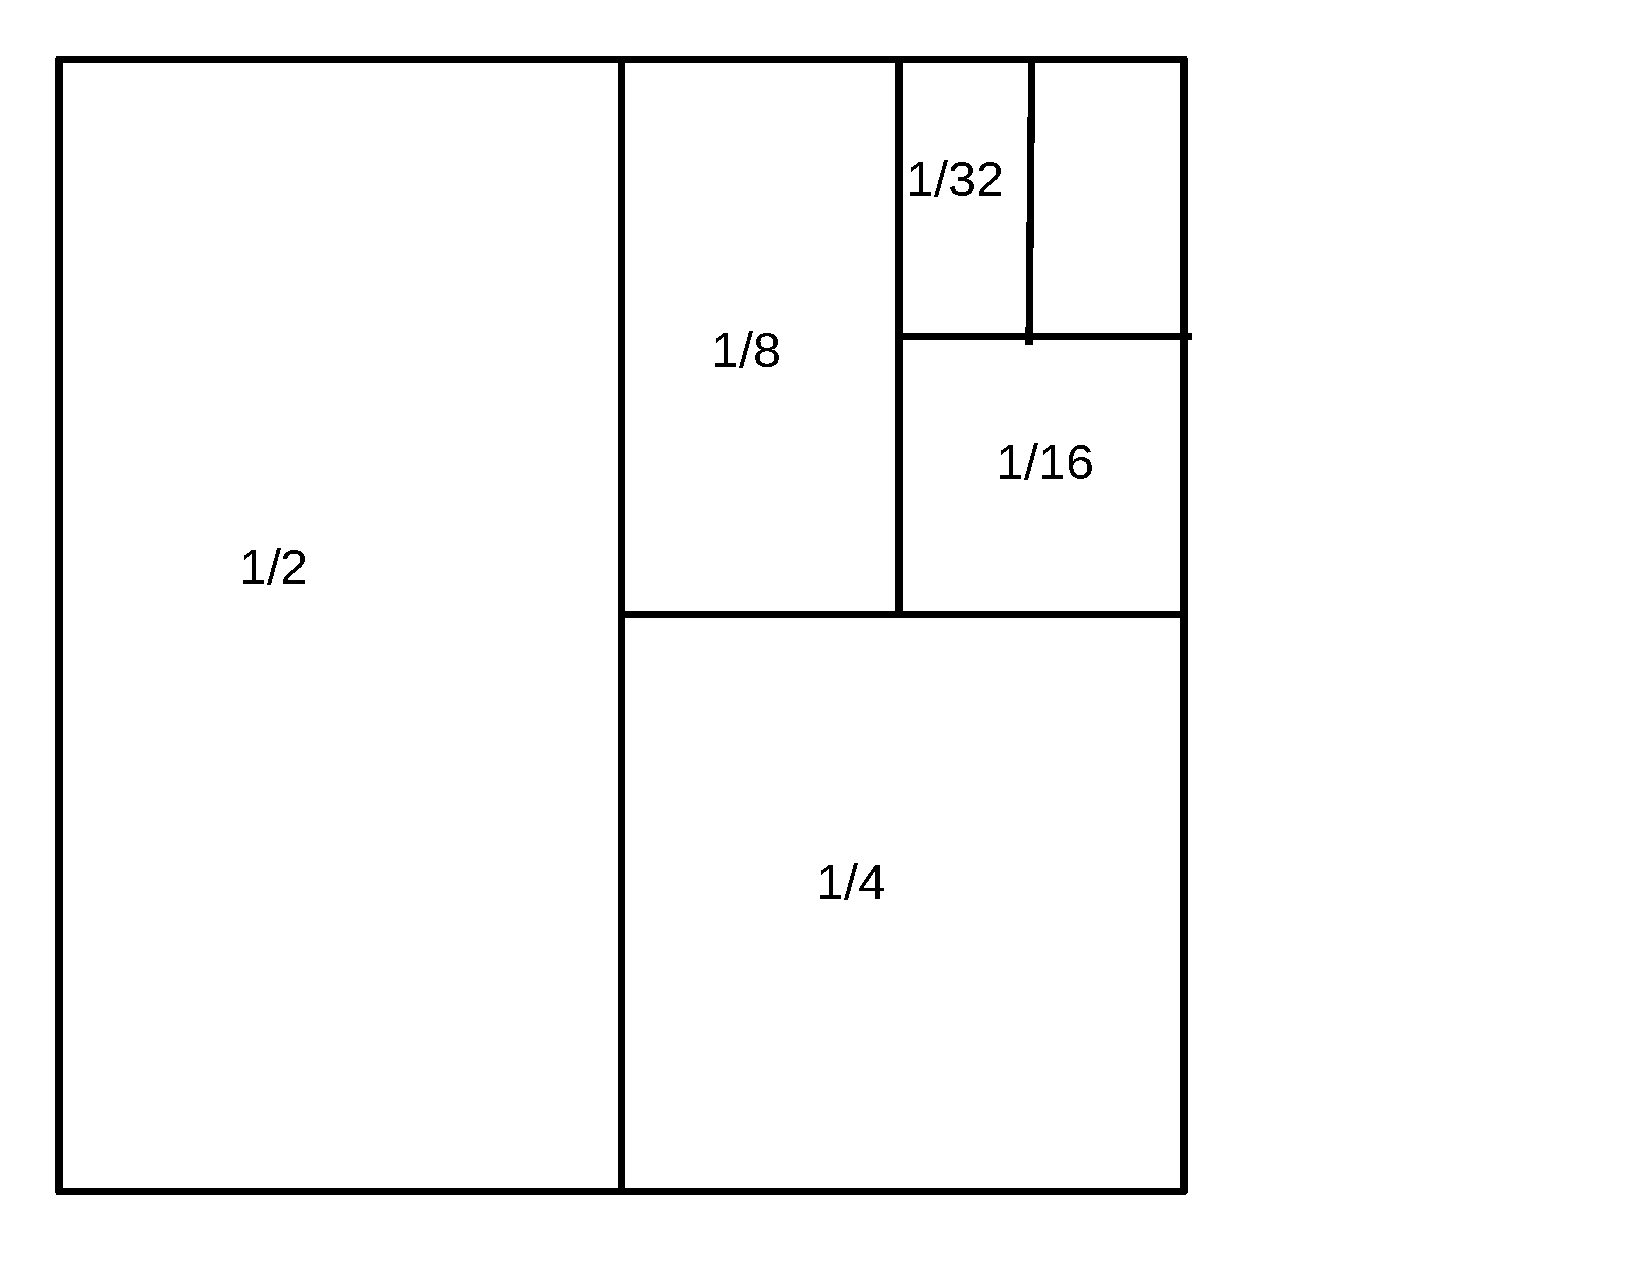
\includegraphics[scale=0.33]{zeno}
\end{center}
\caption{$\sum_{k=1}^{\infty} 2^{-k} = \frac{1}{2} + \frac{1}{4} + \frac{1}{8} + \cdots =1$\label{fig:zeno}}
\end{figure}

\subsubsection{Exercises}
\begin{enumerate}
\item Prove that, if  $\sum_{k=0}^{\infty} b_k$ converges, we must have $\lim b_k = 0$.
\item Evaluate $0.73737373\cdots$ (i.e. express it as a fraction).
\item Prove (assuming convergence) that $c\sum_{k=0}^{\infty} b_k = \sum_{k=0}^{\infty} cb_k$.
\item Evaluate $\sum_{k=0}^{\infty} x^{2k} = 1 + x^2 + x^4 + x^6 + \cdots$ assuming $-1<x<1$.
\item Evaluate $\sum_{k=0}^{\infty} kx^k = x + 2x^2 + 3x^3 + \cdots$ assuming $-1<x<1$. (You cannot get this directly from theorem \ref{thm:geometricSeries}, you will need to work out an expression for the partial sums)
\item Evaluate $\sum_{k=1}^{\infty} \frac{1}{k(k+1)}$. (Forget about theorem \ref{thm:geometricSeries}, just find an expression for the partial sums)
\item The sum (\ref{eq:Zeno}) has an interesting interpretation in terms of probability. If we repeatedly flip a fair coin, what is the probability that we will eventually get ``heads"? One-half is the chance of getting heads immediately, $1/4$ is  the probability of tails then heads, and $2^{-k}$ is the probability that heads first appears at the $k^{\mbox{th}}$ flip: the sum tells us that the probability of eventually seeing heads, if we can flip an unlimited number of times, is one. Does this make sense? By the same reasoning, what is the probability of eventually seeing heads if we repeatedly toss a coin which is biased so that heads appears with probability only $1/3$?
\end{enumerate}

\subsection{Divergent Series}
{\color{red}Harmonic. Exercises on simple variants of harmonic.} 

%At this point what matters is to present more interesting examples of sequences,
%lead this into justification for least-upper-bound assumption, Cauchy sequences (starting with emphasis on sequences with all terms positive).
%But also point out that if we make up some arbitrary rule for $i$th digit, we have (in general) no better description of what the limit is! And if the terms are not of the right form, we might not even be sure we have the decimal digits right ... !?


\subsection{Convergence of Series}
Representation of numbers as decimal expansions is very closely related to convergent series and geometric series.
In fact, an infinite decimal like $\sqrt{2}=1.4142135623730951\cdots$ is nothing but a convenient shorthand for
\begin{equation}\label{eq:decimalExpansion}
\lim_{n\to\infty} 1 + \frac{4}{10} + \frac{1}{100} + \frac{4}{1000} + \frac{2}{10000} + \frac{1}{100000} + \frac{3}{1000000} + \cdots +\frac{d_n}{10^n}
\end{equation}
where $d_n$ is the $n^{\mbox{th}}$ digit. But this raises some surprisingly subtle questions. We always take it for granted that \emph{any} list of digits will define a number -- in the terminology of the previous chapter, we assume that \emph{all sequences of the above form are convergent}. Since we know that many sequences diverge and that it is not always easy to tell, it seems we are assuming quite a lot! But the geometry of the number line makes the assumption thoroughly compelling. We naturally equate ``number" with ``a point on the line"; whenever we add a new digit, we are confining our supposed number/point to an ever-smaller part of the line:
\begin{equation*}\begin{array}{ccc}
1.4 < &\sqrt{2} &< 1.5\\
1.41 < &\sqrt{2} &< 1.42\\
1.414 < &\sqrt{2} &< 1.415
\end{array}\end{equation*}
et cetera. When we ``go to infinity", there is no ambiguity about where this point/number must be. We cannot, say, be left with two candidate points separated by a distance of $10^{-1000}$: after fixing the first 1001 digits, the range of possible values will be narrower than that. Indeed, the boldness of our assumption lies entirely in  the opposite direction, in assuming that the number line is in some sense ``full", so there cannot be a sequence of digits that somehow manages to cut out everything, leaving us with no points at all.

The ``fullness" of the line truly is an assumption, because there is nothing in the rules of arithmetic which requires that an irrational number like $\sqrt{2}$ must exist. There is surely no rule that says every equation must have a solution; if there is no real $x$ such that $x=x+1$ or $x^2=-1$, why must there be something to satisfy $x^2=2$? 
If we were to declare that ``number" means rational number -- i.e. a fraction with integer numerator and denominator -- we would encounter no logical problems at all, since the operations of arithmetic, applied to rational numbers, can only produce other rational numbers.
%If we ``deny the existence" of irrationals, we end up with a vastly smaller collection of convergent sequences -- too small to really be interesting -- but the definition of convergence still makes sense.

Take a careful look at the Babylonian square-root algorithm from section \ref{sec:MeaningOfLimits}: we never actually proved that $X$ has a square root, we only proved that \emph{if} $X$ has a square root, the sequence $r_n$ must converge to it.

Our confidence in the existence of things like $\sqrt{2}$ comes from geometry; the diagonal of a 1-by-1 square can be nothing else. This follows from the Pythagorean theorem -- or more simply from diagram \ref{fig:sqrt2}.  And we cannot limit our geometric intuition to lines; we feel just as strongly that any curve could be ``unrolled" into a line segment, and so must have a numeric length -- hence $\pi$ must be a number because it is the circumference of a circle with diameter $1$.
\begin{figure}
\begin{center}
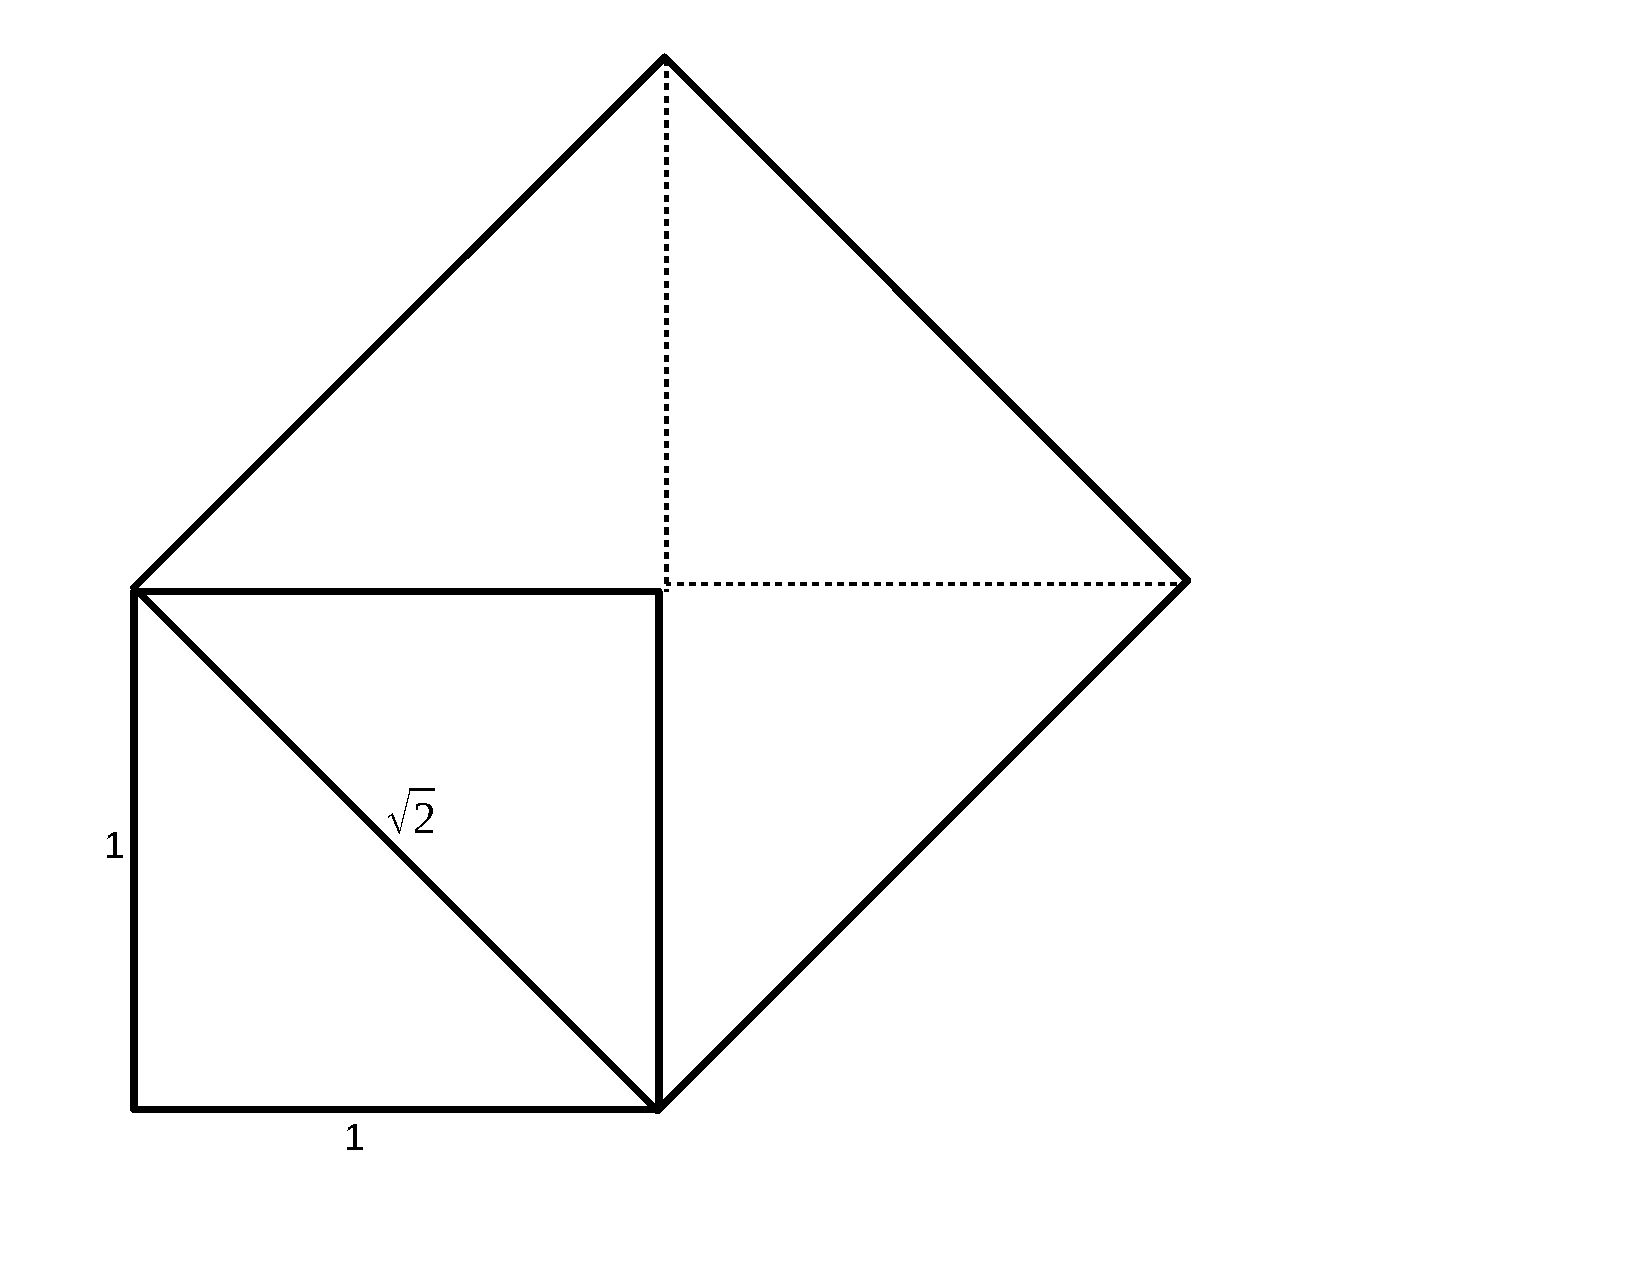
\includegraphics[scale=0.33]{sqrt2}
\end{center}
\caption{Area of the larger square is four triangles, i.e. 2, so its side is the square root of 2\label{fig:sqrt2}}
\end{figure}

We will, in fact, assume that decimal expansions always converge, but we will state that assumption in a rather different form; one which is more useful for proving theorems and which is not tied to the particular notation we use for writing numbers. Before that we must first introduce another central concept of calculus: continuity.
%At that point we will be faced with a rather substantial collection of observations which seem like they must be true, but cannot be proved without assuming the fullness of the number line.
For now we will just prove (as an exercise) a theorem which completely settles which decimals are rational and which are not.
%As in the first chapter, we have begun by focusing on the familiar convention of writing numbers as possibly infinite decimal expansions, but  we actually want to reason about quantities in a way that is not tied to the notation we use to write them. And then we will be done making assumptions; all further results will follow from elementary arithmetic, the Archimedean property, and our to-be-stated assumption about convergence.
%We could in fact \emph{define} a real number to be a sequence of digits; then could define addition/multiplication by giving the rules for how to perform these operations and so on. 

\subsubsection{Exercises}
\begin{enumerate}
\item Prove that if an infinite series of the form
\begin{equation}
\sum_{n=1}^{\infty} \frac{d_n}{10^n}
\end{equation}
converges, the sum must be $<=1$
\item The infinite decimal $0.d_1d_2d_3...$ is  \emph{ultimately periodic} if there are integers $t\geq 0,p\geq 1$ such that $d_{i+p}=d_{i}$ whenever $i>t$; in other words, after an  arbitrary initial segment of length $t$, we keep repeating the same pattern of $p$ digits. Prove that every ultimately periodic decimal represents a rational number.
\item Prove the converse: every rational number has an ultimately periodic decimal representation. (Consider using long division to get one digit after another; what would cause the sequence of digits to become periodic?)
\item Would these two results be any different if we used a base other than ten?
\end{enumerate}


{\color{red}
 \subsection{Convergence Tests}
 Put convergence tests in separate chapter, after derivatives.}
 %Do not need full details of all tests for first draft, but must decide exactly how to formulate Cauchy property and suggest flavor of how this section should look.
%Here is where we have do deal with pure existence of sums we cannot evaluate, so we must make explicit something like the least-upper-bound assumption; given the way we have developed the material, it is better to take convergence of Cauchy sequences as our axiom.
%
%Spivak has the following (skipping the integral test of course): look closely at proofs (exactly where is LUB axiom used?). In place of integral test should be able to manipulate bounds on sum of $x^{-p}$? i.e. approximate the integral; integrals are just expressions for approximate partial sums
%
%\begin{itemize}
%\item comparison (441); this is direct application of LUB; for us it should be the motivation to assume that limits exist even when we cannot evaluate them
%\item ratio (443); this is basically applying comparison test against geometric
%\item Leibniz (448) - again just a careful application of sup/inf/lub et cetera.
%\item product of series (454); might skip this since we have already delayed derivatives so long!
%\end{itemize}
